\documentclass[main]{subfiles}

\begin{document}

\section{Introduction}
\subsection{How this script works}
% Make reference to useful learning materials such as Herlihy, Sophormic Intro and lecture slides/exercises
As mentioned in the disclaimer, this script is not meant to serve as a replacement for the lecture materials presented during the semester. However, this script does try to summarize the material with complementary exercises and examples. The exercises are inspired by former exam questions, but also include some other questions which might occur. The examples are simply meant to re-enforce the reader's understanding of the topics.\\[3mm]
This script was heavily inspired by ''The Art of Multiprocessor Progamming'' by Maurice Herlihy and Nir Shavit and by ''A Sophomoric Introduction to Shared-Memory Parallelism and Concurrency'' by Dan Grossman. Those who are interested in the subject and would like to read more or who feel that this script and the lecture materials didn't manage to cover the subject matter well enough will find these books to be good places to start.

\subsection{Parallelism vs. Concurrency}
The lecture and also this script are organized around a fundamental distinction between \textit{concurrency} and \textit{parallelism}. The definitions of these terms are not universal and many people use them differently. Nonetheless, these definitions are the most generally accepted and making the distinction is important to facilitate discussions on the subject.\\[3mm]
\textit{Parallel programming} is about using additional computational resources to solve a problem faster. 
\begin{example}
    Consider the trivial problem of summing up all numbers in an array. As far as we know, there is no sequential algorithm that can do better than $\Theta(n)$ time. Suppose instead we had 4 processors. We could then produce the result (hopefully) 4 times faster by partitioning the array into 4 segments, having each processor sum one segment, and combining the results with an extra 3 additions.
\end{example}
\textit{Concurrent Progamming} is about correctly and efficiently controlling access by multiple threads to shared resources.
\begin{example}
    Suppose we had several cooks (processes) working in a kitchen and they had some form of shared resource, e.g. an oven. Of course, it's important that a cook doesn't put a zucchini herb casserole in the oven unless the oven is empty. If the oven is not empty, we could keep checking until it is empty. In Java, you might write somehing like: 
    \begin{figure}[H]
        \centering
        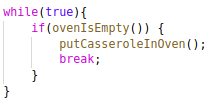
\includegraphics[scale=0.45]{Casserole.png}
    \end{figure}
    Unfortunately, code like this won't work when we have several threads run it at the same time, i.e. when we have several cooks. Problems like these are the primary complication in concurrent programming. Both cooks might observe the oven to be empty and then both put a casserole in, ruining both dishes in the process. We therefore need to think of ways to check if the oven is empty and put the casserole in without any other thread interfering in the mean time.
\end{example}
It's all-too-common for a conversation to become muddled because one person is thinking about parallelism, while the other is thinking about concurrency.\\[3mm]
In practice, the distinction between parallelism and concurrency is not absolute.  Many programs have aspects of each. Suppose you had a huge array of values you wanted to insert into a hash table. From the perspective of dividing up the insertions among multiple threads, this is about parallelism. From the perspective of coordinating access to the hash table, this is about concurrency. Also, parallelism does typically need some coordination: even when adding up integers in an array we need to know when the different threads are done with their chunk of the work.\\[3mm]
It's generally believed that parallelism is an easier concept to start with and we've ordered the chapters accordingly.

\subsection{Basic Threads}
Before writing any parallel or concurrent programs, we need some way of making multiple things happen at once and some way for those different things to communicate.\\[3mm]
The programming model we will assume is explicit threads with shared memory. A thread is like a running sequential program, but one thread can create other threads that are part of the same program and those threads can create more threads, etc. Two or more threads can communicate by writing and reading fields of the same object. They can see the same objects because we assume memory to be shared among them.\\[3mm]
Conceptually, all the threads that have been started but not yet terminated are ''running at once'' in a program (we can't tell the difference). In reality, they may be running at any particular moment, as there may be more threads than processors or a thread may be waiting for something to happen before it continues. When there are more threads than processors, it's up to the Java implementation, with help from the underlying operating system, to find a way to let the threads ''take turns'' using the available processors. This is called \textit{scheduling} and is a major topic in operating systems. All we need to care about is that it's not under our control: We create the threads and the system schedules them.\\[3mm]
We will now discuss some Java specifics for exactly how to create a new thread in Java. The details vary in different languages. In addition to creating threads, we will need other language constructs for coordinating them. For example, for one thread to read the result of another thread's computation, the reader often needs to know the writer is done.\\[3mm]
To create a new thread in Java requires that you define a new class and then perform two actions at run-time:
\begin{enumerate}
    \item Define a subclass of \texttt{java.lang.Thread} and override the \texttt{public} method \texttt{run}, which takes no arguments and has return type \texttt{void}. The \texttt{run} method will act like ''main'' for threads created using this class. It must take no arguments, but the example below shows how to work around this inconvenience.
    \item Create an instance of the class created in step 1. Note that this doesn't create a running thread. It just creates an object.
    \item Call the \texttt{start} method of the object you created in step 2. This step does the ''magic'' creation of a new thread. That new thread will execute the \texttt{run} method of the object. Notice that you do not call \texttt{run}; that would just be an ordinary method call. You call \texttt{start}, which makes a new thread that runs \texttt{run}. The new thread terminates when its \texttt{run} method completes.
\end{enumerate}
\begin{example}
    Here is a useless Java program that starts with one thread and then creates 20 more threads:
    \begin{figure}[H]
        \centering
        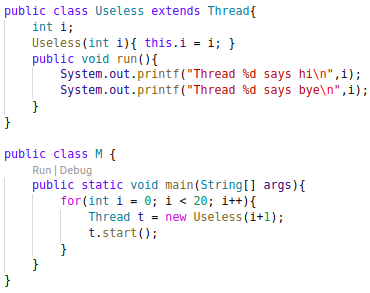
\includegraphics[scale=0.45]{Useless.png}
    \end{figure}
    When running this program, it will print 40 lines of output, the order of which we cannot predict. In fact, if you run the program multiple times, you will probably see the output appear in different orders every run. This showcases that there is no guarantee that threads created earlier will run earlier. Therefore, multithreaded programs are \textit{nondeterministic}. This is an important reason why multithreaded programs are much harder to test and debug.\\[3mm]
    We can also see how this program worked around the rule that \texttt{run} isn't allowed to take any arguments. Any ''arguments'' for the new thread are passed via the constructor, which then stores them in fields so that \texttt{run} can later access them.
\end{example}
We mentioned previously that we'd like to make a thread wait before reading a value until another thread has finished its computations, i.e. its \texttt{run} method. We can do this with the \texttt{join} keyword, which we'll introduce through another somewhat useless example.
\begin{example}
    Here is a Java program that starts with one thread which spawns 20 more threads and waits for all of them to finish.
    \begin{figure}[H]
        \centering
        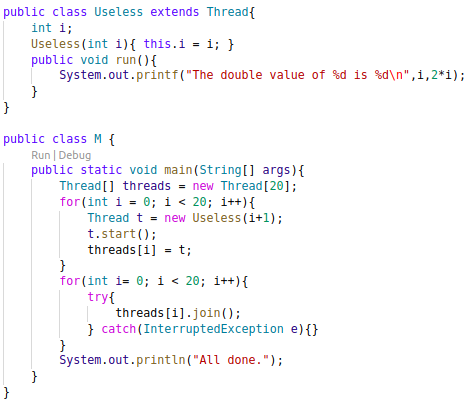
\includegraphics[scale=0.45]{Useless2.png}
    \end{figure}
    The \texttt{join} method can throw an \texttt{InterruptedException}, which means we need to wrap it in a try-catch block.
\end{example}

\subsubsection{Thread states}
If we want to be able to talk about the effects of different thread operations, we need some notion of \textit{thread states}. In short, a Java thread typically goes through the following states:
\begin{itemize}
    \item \textit{Non-Existing}: Before the thread is created, this is where it is. We don't know too much about this place, as it's not actually on this plane of reality, but it's somewhere out there.
    \item \textit{New}: Once the \texttt{Thread} object is created, the thread enters the new state.
    \item \textit{Runnable}: Once we call \texttt{start()} on the new thread object, it becomes eligible for execution and the system can start scheduling the thread as it wishes.
    \item \textit{Blocked}: When the thread attempts to acquire a lock, it goes into a blocked state until it's actually obtained the lock, upon which it returns to a runnable state. In addition, calling the \texttt{join()} method will also transfer at thread into a blocked state.
    \item \textit{Waiting}: The thread can call \texttt{wait()} to go into a waiting state. It'll return to a runnable state once another thread calls \texttt{notify()} or \texttt{notifyAll()} and the thread is removed from the waiting queue.
    \item \textit{Terminated}: At any point during execution we can use the \texttt{interrupt()} to signal the thread that it should stop execution. It will then transfer to a terminated state. Note that when the thread is in a runnable state, it needs to check whether its interrupted flag is set itself, it won't transfer to the terminated state automatically. Of course, exiting the \texttt{run} method is equivalent to entering a terminated state. Once the garbage collector realizes that the thread has been terminated and is no longer reachable, it will garbage collect the thread and it will return to a non-existing state, completing the cycle.
\end{itemize}

\subsection{Bad Interleavings and Data Races}
A \textit{race condition} is a mistake in your program such that whether the program behaves correctly or not depends on the order that the threads execute. Race conditions are very common bugs in concurrent programming that, by definition, do not exist in sequential programming. We distinguish two types of race conditions.\\[3mm]
One kind of race condition is a \textit{bad interleaving}. The key point is that ''what is a bad interleaving'' depends entirely on what you are trying to do. Whether or not it is okay to interleave two bank-account withdraw operations depends on some specification of how a bank is supposed to behave.
\begin{example}
    Suppose we have the following implementation of a \texttt{peek} operation on a concurrent stack.
    \begin{figure}[H]
        \centering
        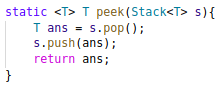
\includegraphics[scale=0.45]{peekWrong.png}
    \end{figure}
    \noindent Assume that the \texttt{pop} and \texttt{push} methods are implemented correctly. While \texttt{peek} might look like it's implemented correctly, the following interleaving might occur:
    \begin{figure}[H]
        \centering
        \begin{subfigure}{.5\textwidth}
            \centering
            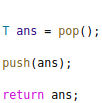
\includegraphics[scale=0.45]{BadInterleaving_1.png}
            \captionsetup{labelformat=empty}
            \caption{Thread 1 (\texttt{peek)}}
        \end{subfigure}%
        \begin{subfigure}{.5\textwidth}
            \centering
            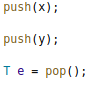
\includegraphics[scale=0.45]{BadInterleaving_2.png}
            \captionsetup{labelformat=empty}
            \caption{Thread 2}
        \end{subfigure}
    \end{figure}
\end{example}
A \textit{data race} is a specific kind of race condition that is better described as a ''simultaneous access error'', although nobody uses that term. There are two kinds of data races:
\begin{itemize}
    \item When one thread might read an object field at the same moment that another thread writes the same field.
    \item When one thread might write an object field at the same moment that another thread also writes the same field.
\end{itemize}
\noindent Notice it is not an error for two threads to both read the same object field at the same time.\\[3mm]
Our programs must never have data races even if it looks like a data race would not cause an error - if our program has data races, the execution of your program is allowed to do very strange things.
\begin{example}
    Let's consider a very simple example.
    \begin{figure}[H]
        \centering
        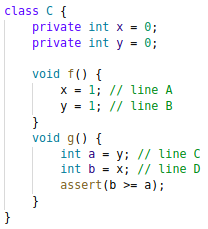
\includegraphics[scale=0.45]{DataRace.png}
    \end{figure}
    Notice that \texttt{f} and \texttt{g} are not synchronized, leading to potential data races on fields \texttt{x} and \texttt{y}, Therefore, it turns out that the assertion in \texttt{g} can fail. But there is no interleaving of operations that justifies the assertion failure, as can be seen through a proof by contradiction: \\[3mm]
    \quad Assume the assertion fails, meaning \texttt{!(b$>=$a)}. Then \texttt{a==1} and \texttt{b==0}. Since \texttt{a==1}, line B happened before line C. Since A must happen before B, C must happen before D, and ''happens before'' is a transitive relation, A must happen before D. But then \texttt{b==1} and the assertion holds.\\[3mm]
    There is nothing wrong with the proof except its assumption that we can reason in terms of ''all possible interleaving'' or that everything happens in certain orders. We can reason this way only if the program has no data races.
\end{example}

\subsection{Other Models}
We've introduced a programming model of explicit threads with shared memory. This is, of course, not the only programming model for concurrent or parallel programming. Shared memory is often considered convenient because communication uses ''regular'' reads and writes of fields to objects . However, it's also considered error-prone because communication is implicit; it requires deep understanding of the code/documentation to know which memory accesses are doing inter-thread communication and which are not. The definition of shared-memory programs is also much more subtle than many programmers think because of issues regarding data races, as discussed in the previous section.\\[3mm]
Three well-known, popular alternatives to shared memory are presented in the following. Note that different models are better suited for different problems. Models can be abstracted and built of top each other as we wish or we can use multiple models in the same program (e.g. MPI with Java).\\[3mm]
\textit{Message-passing} is the natural alternative to shared memory. In this model, we have explicit threads, but they do not share objects. To communicate, there is a seperarte notion of a message, which sends a copy of some data to its recipient. Since each thread has its own objects, we do not have to worry about other threads wrongly updating fields. But we do have to keep track of different copies of things being produced by messages. When processes are far apart, message passing is likely a more natural fit, just like when you send email and a copy of the message is sent to the recipient.\\[3mm]
\textit{Dataflow} provides more structure than having ''a bunch of threads that communicate with each other however they want.'' Instead, the progammer uses primitives to create a directed acyclic graph. A node in the graph performs some computation using inputs that arrive on its incoming edges. This data is provided by other nodes along their outgoing edges. A node starts computing when all of its inputs are available, something the implementation keeps track of automatically.\\[3mm]
\textit{Data parallelism} does not have explicit threads or nodes running different parts of the program at different times. Instead, it has primitives for parallelism that involve applying the same operation to different peices of data at the same time. For example, you would have a primitive for applying some function to every element of an array. The implementation of this primitive would use parallelism rather than a sequential for-loop. Hence all the parallelism is done for you provided you can express your program using the available primitives.

\end{document}